% Options for packages loaded elsewhere
\PassOptionsToPackage{unicode}{hyperref}
\PassOptionsToPackage{hyphens}{url}
%
\documentclass[
]{book}
\usepackage{amsmath,amssymb}
\usepackage{lmodern}
\usepackage{ifxetex,ifluatex}
\ifnum 0\ifxetex 1\fi\ifluatex 1\fi=0 % if pdftex
  \usepackage[T1]{fontenc}
  \usepackage[utf8]{inputenc}
  \usepackage{textcomp} % provide euro and other symbols
\else % if luatex or xetex
  \usepackage{unicode-math}
  \defaultfontfeatures{Scale=MatchLowercase}
  \defaultfontfeatures[\rmfamily]{Ligatures=TeX,Scale=1}
\fi
% Use upquote if available, for straight quotes in verbatim environments
\IfFileExists{upquote.sty}{\usepackage{upquote}}{}
\IfFileExists{microtype.sty}{% use microtype if available
  \usepackage[]{microtype}
  \UseMicrotypeSet[protrusion]{basicmath} % disable protrusion for tt fonts
}{}
\makeatletter
\@ifundefined{KOMAClassName}{% if non-KOMA class
  \IfFileExists{parskip.sty}{%
    \usepackage{parskip}
  }{% else
    \setlength{\parindent}{0pt}
    \setlength{\parskip}{6pt plus 2pt minus 1pt}}
}{% if KOMA class
  \KOMAoptions{parskip=half}}
\makeatother
\usepackage{xcolor}
\IfFileExists{xurl.sty}{\usepackage{xurl}}{} % add URL line breaks if available
\IfFileExists{bookmark.sty}{\usepackage{bookmark}}{\usepackage{hyperref}}
\hypersetup{
  pdftitle={Memphis Code Enforcement},
  pdfauthor={Sarah Johnson},
  hidelinks,
  pdfcreator={LaTeX via pandoc}}
\urlstyle{same} % disable monospaced font for URLs
\usepackage{color}
\usepackage{fancyvrb}
\newcommand{\VerbBar}{|}
\newcommand{\VERB}{\Verb[commandchars=\\\{\}]}
\DefineVerbatimEnvironment{Highlighting}{Verbatim}{commandchars=\\\{\}}
% Add ',fontsize=\small' for more characters per line
\usepackage{framed}
\definecolor{shadecolor}{RGB}{248,248,248}
\newenvironment{Shaded}{\begin{snugshade}}{\end{snugshade}}
\newcommand{\AlertTok}[1]{\textcolor[rgb]{0.94,0.16,0.16}{#1}}
\newcommand{\AnnotationTok}[1]{\textcolor[rgb]{0.56,0.35,0.01}{\textbf{\textit{#1}}}}
\newcommand{\AttributeTok}[1]{\textcolor[rgb]{0.77,0.63,0.00}{#1}}
\newcommand{\BaseNTok}[1]{\textcolor[rgb]{0.00,0.00,0.81}{#1}}
\newcommand{\BuiltInTok}[1]{#1}
\newcommand{\CharTok}[1]{\textcolor[rgb]{0.31,0.60,0.02}{#1}}
\newcommand{\CommentTok}[1]{\textcolor[rgb]{0.56,0.35,0.01}{\textit{#1}}}
\newcommand{\CommentVarTok}[1]{\textcolor[rgb]{0.56,0.35,0.01}{\textbf{\textit{#1}}}}
\newcommand{\ConstantTok}[1]{\textcolor[rgb]{0.00,0.00,0.00}{#1}}
\newcommand{\ControlFlowTok}[1]{\textcolor[rgb]{0.13,0.29,0.53}{\textbf{#1}}}
\newcommand{\DataTypeTok}[1]{\textcolor[rgb]{0.13,0.29,0.53}{#1}}
\newcommand{\DecValTok}[1]{\textcolor[rgb]{0.00,0.00,0.81}{#1}}
\newcommand{\DocumentationTok}[1]{\textcolor[rgb]{0.56,0.35,0.01}{\textbf{\textit{#1}}}}
\newcommand{\ErrorTok}[1]{\textcolor[rgb]{0.64,0.00,0.00}{\textbf{#1}}}
\newcommand{\ExtensionTok}[1]{#1}
\newcommand{\FloatTok}[1]{\textcolor[rgb]{0.00,0.00,0.81}{#1}}
\newcommand{\FunctionTok}[1]{\textcolor[rgb]{0.00,0.00,0.00}{#1}}
\newcommand{\ImportTok}[1]{#1}
\newcommand{\InformationTok}[1]{\textcolor[rgb]{0.56,0.35,0.01}{\textbf{\textit{#1}}}}
\newcommand{\KeywordTok}[1]{\textcolor[rgb]{0.13,0.29,0.53}{\textbf{#1}}}
\newcommand{\NormalTok}[1]{#1}
\newcommand{\OperatorTok}[1]{\textcolor[rgb]{0.81,0.36,0.00}{\textbf{#1}}}
\newcommand{\OtherTok}[1]{\textcolor[rgb]{0.56,0.35,0.01}{#1}}
\newcommand{\PreprocessorTok}[1]{\textcolor[rgb]{0.56,0.35,0.01}{\textit{#1}}}
\newcommand{\RegionMarkerTok}[1]{#1}
\newcommand{\SpecialCharTok}[1]{\textcolor[rgb]{0.00,0.00,0.00}{#1}}
\newcommand{\SpecialStringTok}[1]{\textcolor[rgb]{0.31,0.60,0.02}{#1}}
\newcommand{\StringTok}[1]{\textcolor[rgb]{0.31,0.60,0.02}{#1}}
\newcommand{\VariableTok}[1]{\textcolor[rgb]{0.00,0.00,0.00}{#1}}
\newcommand{\VerbatimStringTok}[1]{\textcolor[rgb]{0.31,0.60,0.02}{#1}}
\newcommand{\WarningTok}[1]{\textcolor[rgb]{0.56,0.35,0.01}{\textbf{\textit{#1}}}}
\usepackage{longtable,booktabs,array}
\usepackage{calc} % for calculating minipage widths
% Correct order of tables after \paragraph or \subparagraph
\usepackage{etoolbox}
\makeatletter
\patchcmd\longtable{\par}{\if@noskipsec\mbox{}\fi\par}{}{}
\makeatother
% Allow footnotes in longtable head/foot
\IfFileExists{footnotehyper.sty}{\usepackage{footnotehyper}}{\usepackage{footnote}}
\makesavenoteenv{longtable}
\usepackage{graphicx}
\makeatletter
\def\maxwidth{\ifdim\Gin@nat@width>\linewidth\linewidth\else\Gin@nat@width\fi}
\def\maxheight{\ifdim\Gin@nat@height>\textheight\textheight\else\Gin@nat@height\fi}
\makeatother
% Scale images if necessary, so that they will not overflow the page
% margins by default, and it is still possible to overwrite the defaults
% using explicit options in \includegraphics[width, height, ...]{}
\setkeys{Gin}{width=\maxwidth,height=\maxheight,keepaspectratio}
% Set default figure placement to htbp
\makeatletter
\def\fps@figure{htbp}
\makeatother
\setlength{\emergencystretch}{3em} % prevent overfull lines
\providecommand{\tightlist}{%
  \setlength{\itemsep}{0pt}\setlength{\parskip}{0pt}}
\setcounter{secnumdepth}{5}
\usepackage{booktabs}
\ifluatex
  \usepackage{selnolig}  % disable illegal ligatures
\fi
\usepackage[]{natbib}
\bibliographystyle{apalike}

\title{Memphis Code Enforcement}
\author{Sarah Johnson}
\date{2021-07-27}

\begin{document}
\maketitle

{
\setcounter{tocdepth}{1}
\tableofcontents
}
\hypertarget{about-the-author}{%
\chapter*{About the Author}\label{about-the-author}}
\addcontentsline{toc}{chapter}{About the Author}

Sarah Johnson is completing her master's in City and Regional Planning from the University of Memphis (expected graduation August 2021).

\hypertarget{intro}{%
\chapter{Introduction}\label{intro}}

In recent years, housing discourse has been dominated by high rates of cost burdenship and the need for affordable rental housing. Less discussed is the need for improved housing quality, particularly in the private rental sector. Housing quality and health have been extensively linked by the public health field, yet tenants who wish to improve their housing quality risk possible retaliation, including increased rents and eviction. Current regulations assume that tenants will take action to report substandard housing, ignoring the risk to a tenant's housing stability. As such, substandard housing is heavily under-reported to code enforcement, often not on their radar till the housing structure is in major disrepair. At this point, the home may be condemned, deemed blighted and demolished, further decreasing the supply of low-rent housing.

This paper seeks to understand the extent of this problem in Memphis. The city has a large percentage of low-income renters, an aging housing stock, a high eviction rate, and high rates of asthma. Particular attention is given to code enforcement policies and data, and how the program has and has not changed over the past twenty years. I conclude with specific recommendations for how to improve code enforcement practices to target the needs of renters.

\hypertarget{housing-and-health}{%
\chapter{Housing and Health}\label{housing-and-health}}

\begin{quote}
The connection between health and dwelling is one of the most important that exists.

\emph{Florence Nightingale}
\end{quote}

\hypertarget{known-links}{%
\section{Known Links}\label{known-links}}

The link between housing and health is extensive and well documented. Occupants of a home are exposed to biologic, chemical, and physical agents that can affect their health and safety \citep[ 63]{cdc2006}. For instance, paint containing lead is known to cause childhood lead poisoning, which lead to the a ban on lead-based paint for residential use in 1978 \citep{cdc2020}.

\hypertarget{respiratory-health}{%
\subsection{Respiratory Health}\label{respiratory-health}}

Asthma, a respiratory disease which causes episodes of wheezing, breathlessness, chest tightness, and coughing, has been linked to exposure to mold or dampness and pests including dust mites, cockroaches, and rodents \citep[ 63]{cdc2006}.

Reviewing the existing literature, \citet{mendell2011} found dampness inside homes was linked to a wide range of respiratory or allergic health effects, including asthma. The authors concluded that prevention and remediation to reduce indoor dampness is urgently needed in a large proportion of the building stock, and such measures could significantly reduce the prevalence of respiratory and allergic disease. \citet{rauh2002} found that cockroach allergen levels are related to the degree of household disrepair, and similarly suggested that public health interventions in housing could reduce allergen exposure.

\hypertarget{healthy-homes}{%
\section{Healthy Homes}\label{healthy-homes}}

Recognizing that ``health, home construction, and home maintenance are inseparable because of their overlapping goals,'' HUD and CDC joined together in 1999 to launch the Healthy Homes Initiative \citep[ 31, 34]{cdc2006}. Many of the basic principles were originally laid out in 1938 by a Committee on the Hygiene of Housing, who provided guidance on the fundamental needs of humans as they relate to housing \citetext{\citealp[ 39]{cdc2006}; \citealp{apha1938}}. The fundamental needs were originally divided into four categories: physiological needs (e.g.~protection from elements), psychological needs (e.g.~adequate privacy), protection against contagion (e.g.~safe water supply), and protection against accidents (e.g.~fire prevention).

The modern Healthy Home Rating System (HHRS) is a list of 29 hazards, categorized in accordance with these needs \citep[ 2]{HHRSover}. The below table lists all the hazards, along with a short description and which populations are most vulnerable to the specific hazard (adopted from \citep{HHRSlst}).

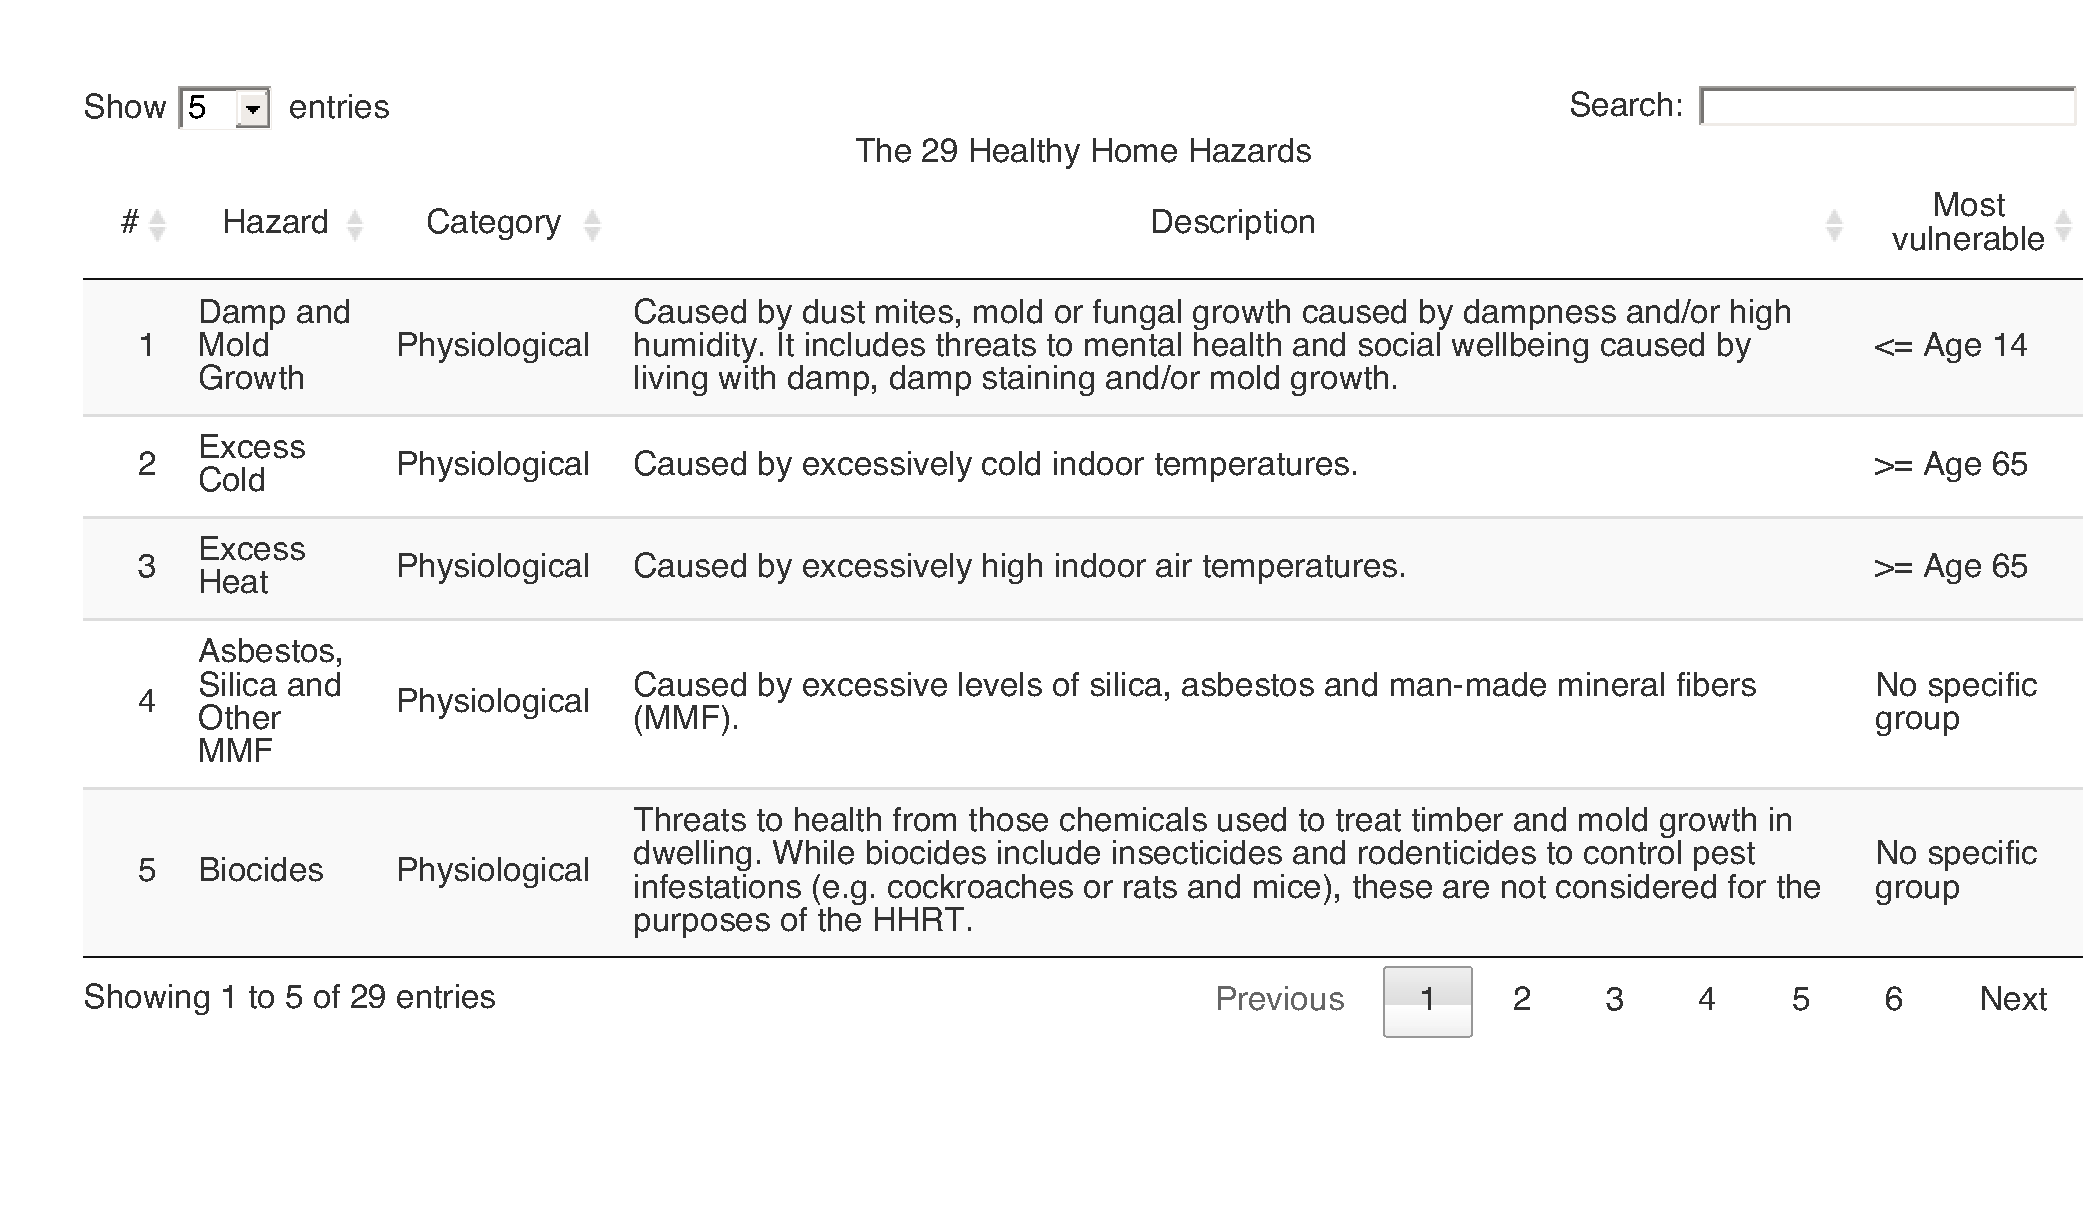
\includegraphics{MA-capstone_files/figure-latex/HHRS-1.pdf}

The HHRS provides a standardized way to identify and rate the risk of home health hazards. Once a hazard is identified, it is further rated according to severity and the effect it is having, or could have, on the occupants. The greater the risk or more serious the outcome, the higher the overall score. The system provides a way to compare risks associated with different types of hazards.

According to \citet{HHRSover}, this system allows local housing and health departments to know which hazards are most serious to the occupants, allowing them to prioritize funding. It also lets local policy makers identify which areas of the community are in greatest need and what health impacts those communities are facing.

\hypertarget{maintenance-in-the-private-rental-market}{%
\section{Maintenance in the Private Rental Market}\label{maintenance-in-the-private-rental-market}}

Health risks caused by larger structural issues can be difficult to implement, particularly for low-income households that rent, as tenants have little or no power to repair such problems. A study of low-income parents of children with asthma found landlords were directly involved in keeping homes in poor condition, even when asked by the tenant to fix the property, and a cycle of fear, poverty, and lack of power compounded to make tenants hesitant to report problems \citep{grineski2010}. Relocating families can reduce health risks, but higher rents associated with safer housing can make it financially difficult or impossible for some families to move \citep{mclaine2006}.

Current regulation of private rental housing quality assumes that tenants will take action to report substandard housing, yet this is often not the case. To understand the disconnect between the law's expectations and reality, \citet{chisholm2018} collected existing qualitative literature to explore power dynamics in the landlord-tenant relationship. The research showed that, for the most part, tenants who ``reported housing quality problems found it a stressful experience, with repairs taking a long time to be carried out, or not at all.'' This experience often impacted future behavior, causing tenants to avoid reporting problems because they did not think it would be effective.

In some cases, tenants would rather move out than work towards a resolution, leaving the issue open for future tenants. In other instances, tenants with low incomes were aware of the lack of alternative housing, causing them to remain silent. Fear of eviction prevented tenants from reporting problems, and this fear was not unfounded; in three of the 15 studies, tenants who reported housing problems were evicted or forced to move. Though laws against retaliatory action might exist, no-cause evictions allow landlords to still remove the tenant from the unit. \citet{chisholm2018} concludes that tenants do not report housing quality problems because the regulation that relies on their reporting fails to protect many tenants.

A wide range of solutions are put forward to improve tenant reporting. Ending no-cause evictions and expanding legal aid can encourage tenants who may have been scared to speak up. Increasing the supply of social or public housing can expand housing options to households most vulnerable to changes in rent. The authors also suggest authorities supervise a web-based reporting system for repair requests, establishing clear records, automated reminders to the landlords, and an opportunity for authorities to step in for unduly slow repairs.

The remainder of this paper seeks to understand the quality of private rental housing in Memphis and systems to report maintenance problems, particularly in cases of landlord neglect.

\hypertarget{memphis}{%
\chapter{Memphis}\label{memphis}}

\hypertarget{health}{%
\section{Health}\label{health}}

In 2015, Memphis was named the asthma capital of America by the Asthma and Allergy Foundation of America \citep{aafa2015}, based on prevalence, risk factors, and medical factors. Recent efforts to reduce the prevalence and risk of asthma have been successful---Memphis's rank has since decreased to 41st in 2021 \citep{aafa2021}.\footnote{The ranking method changed between 2015 and 2021, with fewer factors involved in a city's overall ranking in 2021.} However, Memphis still ranks high in asthma-related mortality, placing 7th of 100 cities.

A recent study comparing pediatric asthma data with property quality information found that asthma prevalence is disproportionately distributed throughout Memphis \citep{shin2018}. Neighborhood blight and inequality were closely associated with childhood asthma and other health problems, leading authors to conclude that effective health interventions should consider involving housing policies and procedures.

\hypertarget{housing}{%
\section{Housing}\label{housing}}

\hypertarget{median-year-built}{%
\subsection{Median Year Built}\label{median-year-built}}

The age of a housing unit can be an indicator that repairs are needed. The below table shows the median age of occupied housing units in the city of Memphis, separated by tenure.

\begin{table}
\caption{\label{tab:medyrblt}City of Memphis: Median year built, occupied housing units}

\centering
\begin{tabular}[t]{l|l|r}
\hline
year & tenure & estimate\\
\hline
2009 & Owner & 1966\\
\hline
2010 & Owner & 1966\\
\hline
2011 & Owner & 1966\\
\hline
2012 & Owner & 1966\\
\hline
2013 & Owner & 1966\\
\hline
2014 & Owner & 1966\\
\hline
2015 & Owner & 1966\\
\hline
2016 & Owner & 1966\\
\hline
2017 & Owner & 1966\\
\hline
2018 & Owner & 1966\\
\hline
2019 & Owner & 1966\\
\hline
\end{tabular}
\centering
\begin{tabular}[t]{l|l|r}
\hline
year & tenure & estimate\\
\hline
2009 & Renter & 1973\\
\hline
2010 & Renter & 1973\\
\hline
2011 & Renter & 1973\\
\hline
2012 & Renter & 1973\\
\hline
2013 & Renter & 1973\\
\hline
2014 & Renter & 1973\\
\hline
2015 & Renter & 1973\\
\hline
2016 & Renter & 1973\\
\hline
2017 & Renter & 1973\\
\hline
2018 & Renter & 1973\\
\hline
2019 & Renter & 1974\\
\hline
\end{tabular}
\end{table}

The Memphis housing stock is aging. The median year built has not (or barely) budged over the past ten years for all occupied homes. The median age of owner-occupied homes is 55 years; for renter-occupied homes, 47 years. The median year built for both owner and renter occupied units is before the ban of lead-based paint in 1978, indicating many homes are at risk for lead poisoning if they have not been remediated.

When we expand our scope from the city limits to the Memphis MSA, there is a noticeable shift in the data, as seen in the table below.

\begin{table}
\caption{\label{tab:unnamed-chunk-6}Memphis MSA: Median year built, occupied housing units}

\centering
\begin{tabular}[t]{l|l|r}
\hline
year & tenure & estimate\\
\hline
2009 & Owner & 1980\\
\hline
2010 & Owner & 1982\\
\hline
2011 & Owner & 1982\\
\hline
2012 & Owner & 1983\\
\hline
2013 & Owner & 1983\\
\hline
2014 & Owner & 1983\\
\hline
2015 & Owner & 1983\\
\hline
2016 & Owner & 1984\\
\hline
2017 & Owner & 1984\\
\hline
2018 & Owner & 1984\\
\hline
2019 & Owner & 1985\\
\hline
\end{tabular}
\centering
\begin{tabular}[t]{l|l|r}
\hline
year & tenure & estimate\\
\hline
2009 & Renter & 1976\\
\hline
2010 & Renter & 1977\\
\hline
2011 & Renter & 1977\\
\hline
2012 & Renter & 1978\\
\hline
2013 & Renter & 1978\\
\hline
2014 & Renter & 1978\\
\hline
2015 & Renter & 1978\\
\hline
2016 & Renter & 1978\\
\hline
2017 & Renter & 1978\\
\hline
2018 & Renter & 1978\\
\hline
2019 & Renter & 1978\\
\hline
\end{tabular}
\end{table}

In the MSA, the median age of renter-occupied homes is 43; for owner-occupied units, 36. This signifies that most new development in the MSA has been for owner-occupied homes outside city limits.

Data on housing quality in the Memphis MSA is available through the 2019 \href{https://www.census.gov/programs-surveys/ahs.html}{American Housing Survey}. As the median age for rental homes is seven years older than for owner-occupied homes in the MSA, we can expect renter-occupied homes to have more deficiencies and problems than owner-occupied homes.

When surveyed on the adequacy of their housing, 14.5\% of renter-occupied units were thought of as inadequate, compared to 10\% of owner-occupied units. This disparity in quality between renter- and owner-occupied households is significant when we compare specific housing problems, as shown in the tables below.\footnote{In the discussions below, ``renters'' refers to renter-occupied units, ``owners'' refers to owner-occupied units, and ``Memphis'' refers to the Memphis MSA.}

\hypertarget{selected-housing-deficiencies}{%
\subsection{Selected Housing Deficiencies}\label{selected-housing-deficiencies}}

\begin{longtable}[]{@{}
  >{\raggedright\arraybackslash}p{(\columnwidth - 10\tabcolsep) * \real{0.52}}
  >{\raggedright\arraybackslash}p{(\columnwidth - 10\tabcolsep) * \real{0.11}}
  >{\raggedright\arraybackslash}p{(\columnwidth - 10\tabcolsep) * \real{0.12}}
  >{\raggedright\arraybackslash}p{(\columnwidth - 10\tabcolsep) * \real{0.04}}
  >{\raggedright\arraybackslash}p{(\columnwidth - 10\tabcolsep) * \real{0.10}}
  >{\raggedright\arraybackslash}p{(\columnwidth - 10\tabcolsep) * \real{0.12}}@{}}
\caption{Selected Housing Deficiencies}\tabularnewline
\toprule
& \textbf{Rent} & & & \textbf{Own} & \\
\midrule
\endfirsthead
\toprule
& \textbf{Rent} & & & \textbf{Own} & \\
\midrule
\endhead
\textbf{Deficiency} & \textbf{Est} & \textbf{Pct} & & \textbf{Est} & \textbf{Pct} \\
Signs of cockroaches in last 12 months & 50.9 & \textbf{22.7\%} & & 44.4 & 15.3\% \\
Signs of mice or rats inside home in last 12 months & 24.4 & 10.9\% & & 32.6 & \textbf{11.3\%} \\
Open cracks or holes (interior) & 14.4 & \textbf{6.4\%} & & 12.1 & 4.2\% \\
Rooms without electric outlets & 6.6 & \textbf{2.9\%} & & 5.0 & 1.7\% \\
Broken plaster or peeling paint (interior) & 5.3 & \textbf{2.4\%} & & 5.8 & 2.0\% \\
Exposed wiring & 3.9 & \textbf{1.7\%} & & 4.5 & 1.6\% \\
Total housing units & 224.0 & - & & 289.7 & - \\
\bottomrule
\end{longtable}

\emph{Source: \href{https://www.census.gov/newsroom/press-releases/2020/2019-american-housing-survey.html}{American Housing Survey} (2019). Estimates in thousands of housing units.}

Renter-occupied units experienced more housing deficiencies than owner-occupied units for all but one of the selected problems.

Pests are prevalent in both owner and renter-occupied units. Renters saw more signs of cockroaches (by 7.4 percentage points), while owners were more likely to sight mice or rats (by 0.4 percentage points). These trends align with national data, where renters were 1.98 times more likely to see cockroaches and owners were 1.17 times more likely to report a rodent sighting \citep{sellner2021}. Compared to national averages, housing units in the Memphis MSA saw slightly fewer rodents (11.1\% vs 11.9\%) and significantly more cockroaches (18.6\% vs.~11.3\%).

Renters were moderately more likely to have open cracks or holes in the interior of their home and to have rooms without electrical outlets. They were also slightly more likely to have decaying interior walls and exposed wiring.

\hypertarget{housing-problems}{%
\subsection{Housing Problems}\label{housing-problems}}

The following table shows the number of units who experience selected housing problems. An estimate of ``S'' denotes a sample too small to meet publication standards or avoid disclosure of identifying information. The total column (``Tot'') is the number of housing units \emph{capable} of experiencing each problem (rather than all housing units). For instance, the total number of units with heating problems only includes units with heating equipment who occupied their unit last winter (excluding units without heating equipment or those who did not occupy their unit last winter).

\begin{longtable}[]{@{}
  >{\raggedright\arraybackslash}p{(\columnwidth - 14\tabcolsep) * \real{0.44}}
  >{\raggedright\arraybackslash}p{(\columnwidth - 14\tabcolsep) * \real{0.08}}
  >{\raggedright\arraybackslash}p{(\columnwidth - 14\tabcolsep) * \real{0.09}}
  >{\raggedright\arraybackslash}p{(\columnwidth - 14\tabcolsep) * \real{0.09}}
  >{\raggedright\arraybackslash}p{(\columnwidth - 14\tabcolsep) * \real{0.03}}
  >{\raggedright\arraybackslash}p{(\columnwidth - 14\tabcolsep) * \real{0.08}}
  >{\raggedright\arraybackslash}p{(\columnwidth - 14\tabcolsep) * \real{0.08}}
  >{\raggedright\arraybackslash}p{(\columnwidth - 14\tabcolsep) * \real{0.09}}@{}}
\caption{Selected Housing Problems}\tabularnewline
\toprule
& & \textbf{Rent} & & & & \textbf{Own} & \\
\midrule
\endfirsthead
\toprule
& & \textbf{Rent} & & & & \textbf{Own} & \\
\midrule
\endhead
\textbf{Problem} & \textbf{Est} & \textbf{Tot} & \textbf{Pct} & & \textbf{Est} & \textbf{Tot} & \textbf{Pct} \\
No flush toilet working some time in last 3 months & 7.0 & 224.0 & \textbf{3.1\%} & & S & 289.7 & - \\
Uncomfortably cold for 24 hours or more & 12.3 & 186.2 & \textbf{6.6\%} & & 10.8 & 278.8 & 3.9\% \\
Fuses or breakers blown in last 3 months & 14.1 & 223.8 & 6.3\% & & 19.3 & 289.7 & \textbf{6.7\%} \\
Water stoppage in last 3 months & 6.4 & 223.8 & \textbf{2.9\%} & & 3.2 & 289.5 & 1.1\% \\
Water leakage from inside structure & 19.5 & 224.0 & \textbf{8.7\%} & & 20.7 & 289.7 & 7.1\% \\
Water leakage from outside structure & 18.9 & 224.0 & 8.4\% & & 25.5 & 289.7 & \textbf{8.8\%} \\
Mold in last 12 months & 11.8 & 224.0 & \textbf{5.3\%} & & 5.8 & 289.7 & 2.0\% \\
Public sewer breakdown in last 3 months & 5.1 & 217.9 & \textbf{2.3\%} & & S & 252.3 & - \\
\bottomrule
\end{longtable}

\emph{Source: \href{https://www.census.gov/newsroom/press-releases/2020/2019-american-housing-survey.html}{American Housing Survey} (2019). Estimates in thousands of housing units.}

Renter-occupied units were overall more likely to experience housing problems and breakdowns than owner-occupied units.

The most common problem for renters and owners was water leakage during the past year. Owners were slightly more likely (by 0.4 percentage points) to experience leakage from outside the structure, such as from the roof, walls, closed windows, or doors. Renters were more likely (by 1.6 percentage points) to experience internal water leakage, such as from a leaky pipe, a broken water heater, or a backed up or overflown fixture. This is likely why renters were more likely to report mold growth within the past year (by 3.3 percentage points).

Heating problems causing households to be uncomfortably cold for at least a day were more common for renter-occupied units (by 2.7 percentage points). Renters were also more likely to experience sanitation problems barely reported by owners. This includes having a public sewer breakdown or having no working toilets at some point in the last three months.

Owners were slightly more likely to recently experience a blown fuse or breaker.

\hypertarget{external-building-conditions}{%
\subsection{External Building Conditions}\label{external-building-conditions}}

The following table shows the number of units experiencing external building problems. This table is limited to single-unit homes, excluding multi-unit homes. Homes with more than one unit are significantly more likely to be renter-occupied. As such, approximately 106,400 rental units were excluded from this table.

\begin{longtable}[]{@{}
  >{\raggedright\arraybackslash}p{(\columnwidth - 10\tabcolsep) * \real{0.55}}
  >{\raggedright\arraybackslash}p{(\columnwidth - 10\tabcolsep) * \real{0.11}}
  >{\raggedright\arraybackslash}p{(\columnwidth - 10\tabcolsep) * \real{0.12}}
  >{\raggedright\arraybackslash}p{(\columnwidth - 10\tabcolsep) * \real{0.04}}
  >{\raggedright\arraybackslash}p{(\columnwidth - 10\tabcolsep) * \real{0.10}}
  >{\raggedright\arraybackslash}p{(\columnwidth - 10\tabcolsep) * \real{0.10}}@{}}
\caption{External Building Conditions}\tabularnewline
\toprule
& \textbf{Rent} & & & \textbf{Own} & \\
\midrule
\endfirsthead
\toprule
& \textbf{Rent} & & & \textbf{Own} & \\
\midrule
\endhead
\textbf{External Building Conditions} & \textbf{Est} & \textbf{Pct} & & \textbf{Est} & \textbf{Pct} \\
Bars on windows & 16.1 & \textbf{16.7\%} & & 22.0 & 7.7\% \\
Broken windows & 7.6 & \textbf{6.5\%} & & 7.8 & 2.7\% \\
Missing roofing material & 7.0 & \textbf{6.0\%} & & 15.5 & 5.4\% \\
Hole in roof & 4.2 & \textbf{3.6\%} & & 6.2 & 2.2\% \\
Missing bricks, siding, or other outside wall material & 3.9 & 3.3\% & & 9.4 & 3.3\% \\
Total housing units (excludes multi-units) & 117.6 & - & & 286.9 & - \\
\bottomrule
\end{longtable}

Source: \href{https://www.census.gov/newsroom/press-releases/2020/2019-american-housing-survey.html}{American Housing Survey} (2019). Estimates in thousands of housing units.

Renters in single-unit homes were significantly more likely to experience external building problems than owner-occupied units, except for missing wall material, which afflicted 3.3\% of both renters and owners. Having bars on windows was especially more common in rental homes (by 9.0 percentage points), as well as having broken windows (by 3.8 percentage points). They were also slightly more likely to have roofing issues, such as missing roofing material or having a hole in the roof.

\hypertarget{summary}{%
\section{Summary}\label{summary}}

Renter-occupied units in Memphis are more likely than owner-occupied units to experience housing issues, and by wider margins. Of the 19 housing quality issues discussed in the three tables above, only three problems were more likely to be experienced by owner-occupied units, and only by a margin of 0.4 percentage points for each problem. Meanwhile, there were 15 problems more common in renter-occupied units, 13 of which had a margin greater than 0.4 percentage points.

\hypertarget{code-enforcement}{%
\chapter{Code Enforcement}\label{code-enforcement}}

\hypertarget{reports}{%
\section{Reports}\label{reports}}

Over the past twenty years, there have been at least two expansive reports offering critiques and criticisms of Memphis code enforcement. While each report aimed to improve code enforcement, the reasons differed---one sought to address crime and safety, the other public health.

The first report, released in April 2001, was distributed by the Memphis Shelby Crime Commission and written by Phyllis Betts, then a professor of sociology at University of Memphis \citep{betts2001}. Input was provided by two other University of Memphis faculty: Betts's husband, the late Richard Janikowski, former chair of the Department of Criminology and Criminal Justice and `father' of Memphis's Blue CRUSH policing \citep{poe2021}; and Susan Roakes, former professor of City and Regional Planning.

The report was built on the ``broken windows'' criminology theory: in deteriorated or declining neighborhoods, physical neglect of ``problem properties'' attracts and aggravates criminal activity. Researchers interviewed inspectors and individuals involved with environmental court, used code enforcement data from 1992-1999, accessed the Shelby County Tax Assessor's database, and conducted visual surveys for selected properties as part of a case study of the Binghamton neighborhood.

The second report, published in 2018, was produced by The Urban Institute \citep{stacy2018}. While the 2001 report focused on property neglect and safety, this report centered on the link between the physical condition of homes and neighborhoods and public health. Planning for the report began shortly after the election of Mayor Jim Strickland in 2016, whose campaign had emphasized blight control \citep{baker2018}. Researchers collaborated with and interviewed members of the newly formed \href{http://memphisfightsblight.com/blight-elimination-steering-team/}{Blight Elimination Steering Team}, a coordinated effort between public, private, and nonprofit agencies to address blight, and the \href{https://www.greenandhealthyhomes.org/location/memphis-tn/}{Green and Healthy Homes Initiative}, a partnership formed between local health care providers and housing and community development organizations to address public health issues related to housing quality.

The report accessed and analyzed data through the \href{http://memphisfightsblight.com/programs/mph/}{Memphis Property Hub}, which offers parcel-level property information, particularly related to blighted, vacant, and foreclosed homes. Code enforcement data from 1999-2017 was used, effectively picking up where the last report ended. Additional data related to public health, safety, and courts were provided by the Shelby County Healthy Department, the Center for Applied Earth Science and Engineering Research department at the University of Memphis, and the Shelby County Environmental Court, respectively.

\hypertarget{findings}{%
\subsection{Findings}\label{findings}}

In a visual survey of the Binghamton neighborhood, \citet{betts2001} found that only about 1 in 5 code violations were reported.

Both reports found the vast majority of code enforcement reports were related to nonstructural issues. \citet{betts2001} reported three out of four properties were cited for non-structural problems such as weeds, junk, and inoperable or abandoned vehicles. It appears this percentage has actually increased overtime; \citet{stacy2018} stated 81\% of all requests concerned the yard or property, rather than the house.

\citet{stacy2018} found service requests were concentrated in areas with single-family homes, and though about half of all requests were for multifamily units, most of these (70 percent) were for duplexes rather than apartment complexes. \citet{betts2001} also found that large multifamily units flew under the radar; at least half of multifamily properties in Binghamton had violations in multiple units, yet code enforcement recorded only eight violations out of 1200 apartment units.

It appears the number of service requests has increased overtime. In 1998, code enforcement received about 10,000 complaints \citep[ 93]{betts2001}, while the Urban Institute reported 53,226 in 2016 \citep[ 51]{stacy2018}. However, this number does not match open data (discussed later in this paper) which reported 30,361 requests in 2016, not excluding duplicates. Nevertheless, it does appear that more requests are being made.

Cases also appear significantly more likely to be taken to court. In 1998, a mere 71 cases from code enforcement were heard by the environmental court \citep[ 49]{betts2001}. In November 2017 alone, 1,095 cases went to environmental court, though the Urban report does not specifically state if all cases were from code enforcement \citep[ 51]{stacy2018}. However, the majority of cases were for single-family homes (64\%), and most were vacant.

\hypertarget{recommendations}{%
\subsection{Recommendations}\label{recommendations}}

Both reports recommend fundamentally changing Memphis code enforcement from a reactive process (responding to citizen reports) to a proactive, strategic system.

\citet{stacy2018} suggests that code enforcement prioritize health-related violations and interior health and safety issues, cemented through the agency's policies and procedures manual. The authors recommend proactive inspections of problem multifamily properties and under-served neighborhoods, and identification of under-reported violations. Multiple technology improvements are recommended, including automatic prioritization of health-related violations and synchronizing of data systems with the Shelby County Department of Health and the environmental court, among others. Also acknowledged is the need to update current landlord/tenant laws to protect tenants from homelessness.

\hypertarget{data}{%
\section{311 Data}\label{data}}

Memphians are able to report problems to code enforcement by calling 311 or submitting a request through an app called \href{https://seeclickfix.com/}{SeeClickFix}, used in hundreds of towns across the nation.

Housing code enforcement data from 2016-present is available through \href{https://data.memphistn.gov/dataset/Service-Requests-since-2016/hmd4-ddta}{Memphis Data Hub}. This page uses a dataset downloaded July 19, 2021. At the time of download, there were 53 columns and 1,232,097 rows. R/RStudio was used to view and analyze the dataset.

Each row of the dataset contains all information for a single request, meaning there are not multiple rows for individual cases (except for duplicates).

Despite the large number of records, only a portion are relevant to this paper. This is because the dataset contains \textbf{all} requests to 311, not just those related to code enforcement. Additionally, many columns contain duplicate or unhelpful information. For instance, there are 23 columns related to location and under the column \texttt{LAST\_UPDATED\_BY}, every single entry is just the number ``460101''.

The dataset can be simplified by filtering for code enforcement data and narrowing the number of columns. In the next section I more thoroughly explain why I chose these columns.

\textbf{NOTE}: A list of all column names is available on the Data Hub site linked above, or in R/RStudio enter \texttt{colnames(Service\_Requests\_since\_2016)}.

\begin{Shaded}
\begin{Highlighting}[]
\NormalTok{CE }\OtherTok{\textless{}{-}}\NormalTok{ Service\_Requests\_since\_2016 }\SpecialCharTok{\%\textgreater{}\%}
  \FunctionTok{filter}\NormalTok{(DEPARTMENT }\SpecialCharTok{==} \StringTok{"Code Enforcement"}\NormalTok{) }\SpecialCharTok{\%\textgreater{}\%}
  \FunctionTok{select}\NormalTok{(}
\NormalTok{    INCIDENT\_NUMBER, }\CommentTok{\#\textquotesingle{} service request (sr) number}
\NormalTok{    PARCEL\_ID, }\CommentTok{\#\textquotesingle{} parcel ID}
\NormalTok{    ADDRESS1, }\CommentTok{\#\textquotesingle{} the street name \& number}
\NormalTok{    REQUEST\_TYPE, }\CommentTok{\#\textquotesingle{} request category}
\NormalTok{    CE\_CATEGORY, }\CommentTok{\#\textquotesingle{} category for CE action}
\NormalTok{    RESOLUTION\_CODE}\SpecialCharTok{:}\NormalTok{RESOLUTION\_SUMMARY, }\CommentTok{\#\textquotesingle{} how the request resolved}
\NormalTok{    REQUEST\_STATUS, }\CommentTok{\#\textquotesingle{} open or closed?}
\NormalTok{    REPORTED\_DATE, }
\NormalTok{    LAST\_MODIFIED\_DATE, }
\NormalTok{    OWNER\_NAME, }\CommentTok{\#\textquotesingle{} assigned code inspector}
\NormalTok{    CREATED\_BY\_USER,}
\NormalTok{    location1 }\CommentTok{\#\textquotesingle{} geocoordinates}
\NormalTok{  )}
\end{Highlighting}
\end{Shaded}

The output is 14 columns and 154,844 rows, significantly easier to work with.

\hypertarget{problems-with-the-dataset}{%
\subsection{Problems with the dataset}\label{problems-with-the-dataset}}

We're ready to begin looking at the data, but before analyzing you should know that there are significant problems with this dataset, including inconsistent and vague data entry, hard-to-filter duplicates, an error causing the wrong address to appear, and more. As such, I was not able to quickly process and analyze this data.

Throughout the dataset, there are \textbf{multiple values that mean the same thing}, like closed and resolved\footnote{Resolved has only been used 72 times, which begs the question of whether it needs to exist at all.}. The \texttt{RESOLUTION\_CODE} field in particular has a handful of codes used for an umbrella of meanings. For instance, 23\% of rows are resolved as ``NJ'' for Not Justified. This may mean an inspector has visited the property and did not see a problem, or there was a wrong address\footnote{INSUF (Insufficient information) is also used for wrong address cases.}, or there was a problem and it's been fixed, or there was a problem but it wasn't related to code enforcement; but in most cases there is no further explanation given. There are similar problems for codes tagged CVOM (COMP. V.O. - Miscellaneous, 9\% of all cases), CVOID (Closed Void, 4\% cases), CO (Closed Other, 3\%), and Other (1\%). Together, these codes make up \underline{40\%} of all code enforcement cases.

Another field with this problem is \texttt{REQUEST\_TYPE}. From 2016 to present, 29\% of all requests were simply listed as ``Code Miscellaneous''.

Some problems are caused by a \textbf{lack of updates} on behalf of inspectors. A file may never be closed in the system, even though the inspector is finished looking at the case. There are 779 active cases created in 2018 or earlier (at least 2.5 years old) and it is unclear if some are in a lengthy legal battle or were simply never updated.

There are many many \textbf{duplicated entries}. It's hard to determine exactly how many, because the duplicates will have unique values under \texttt{INCIDENT\_NUMBER} and slightly different date/times. For this reason it is hard to filter out without accidentally omitting multiple legitimate entries under the same property. Also, any entries that were created in error are kept in the system. This leads to inspectors frequently entering ``see sr\#xxxxxx'' in the \texttt{RESOLUTION\_SUMMARY}, referring to a different \texttt{INCIDENT\_NUMBER} that contains the correct file.\footnote{There are 6,391 instances of a \texttt{RESOLUTION\_SUMMARY} mentioning ``sr'', and nearly all of these rows are likely to be duplicates.} There is also a code specifically for duplicate entries that already have an active file, JA (Justified, Active already file), which has been used 6,588 times, though other codes are known to be used for this same problem.

\textbf{Other problems are more major.} It appears that SeeClickFix (SCF), a program used to allow users to create requests, can cause the \textbf{wrong address} to be entered into the system. There is no warning given for this error. When I attempted to sort addresses with the most violations, the top address does not actually exist in the city of Memphis. The inspectors know this and they seem to be able to view the correct address in SCF, and sometimes (but not often) they will manually write this address in the \texttt{RESOLUTION\_SUMMARY}. It is unclear how many addresses have this problem, but it does affect multiple addresses. As a researcher, I feel nervous conducting research on data with such obvious errors.

Each row is meant to hold all information for a single case. There is also only one column for inspectors to manually enter notes: \texttt{RESOLUTION\_SUMMARY}. This column has become a \textbf{catch-all} for legitimate information, though it is also NA in 23\% of rows. In many other cases there is little elaboration, or the \texttt{RESOLUTION\_CODE\_MEANING} is simply repeated. Despite having eight different date columns, it is very common for dates to be entered here with the notes. Because this field is typed, typos are not-uncommon---tenant is spelled ``tennant'' 51 times, with many other variations such as ``tenenat'', ``tenet'', ``teneant'' and ``tenent''. Other times a tenant is referred to as a ``resident''. These variances make it difficult to find all instances of keywords.

Lastly, there are also obvious \textbf{privacy issues} included in the field, such as the full name and phone numbers of individuals.

\hypertarget{duplicates-errors}{%
\subsection{Duplicates \& Errors}\label{duplicates-errors}}

Searching for duplicates is made difficult by the large number of errors in the dataset. This is made clear when we begin searching for addresses with the most service requests.

\begin{Shaded}
\begin{Highlighting}[]
\NormalTok{CE }\SpecialCharTok{\%\textgreater{}\%} \FunctionTok{count}\NormalTok{(ADDRESS1) }\SpecialCharTok{\%\textgreater{}\%} \FunctionTok{arrange}\NormalTok{(}\FunctionTok{desc}\NormalTok{(n))}
\end{Highlighting}
\end{Shaded}

\begin{verbatim}
## # A tibble: 73,772 x 2
##    ADDRESS1               n
##    <chr>              <int>
##  1 <NA>                 547
##  2 746 CHAPEL ST        194
##  3 45 S IDLEWILD ST     117
##  4 1490 HUGENOT ST       88
##  5 3923 JACKSON AVE      76
##  6 102 PLAINVIEW ST      73
##  7 400 S HIGHLAND ST     72
##  8 1081 COURT AVE APT    71
##  9 3373 STEVE RD         50
## 10 810 WASHINGTON AVE    46
## # ... with 73,762 more rows
\end{verbatim}

There are 194 entries listed under the address 746 Chapel St, an address that does not seem to exist in Memphis (there is a Chapel \underline{Rd}, but no 746). Reviewing the \texttt{RESOLUTION\_SUMMARY} reveals the address to be a catch all of errors. Sometimes a different address or a business name is written in the \texttt{RESOLUTION\_SUMMARY}, indicating the results we are seeing is not the same as what was originally entered, yet code inspectors may be able to view the correct address. It is likely best to remove this address from any analysis involving location.

At 1490 Hugenot St, there are 117 requests, but this property appears to have the same problem as 746 Chapel. This is revealed by certain entries in the \texttt{RESOLUTION\_SUMMARY} including ``The correct address is xxx Summer Ave.'' and ``INSUFFICIENT INFORMATION WRONG ADDRESS SUBMITTED BY SEECLICKFIX'' (SeeClickFix, or SCF, is listed as the request creator for all but five entries at this address).

As for 45 S Idlewild, this is a valid location (an apartment complex) with 117 service requests. A closer look shows three people made 20 requests on February 1, 2019. Yet as discussed below, it is not clear if we should trust the information seen in \texttt{CREATED\_BY\_USER}.

When we look closer at \emph{who} is making complaints to code enforcement, it at first seems a few people are creating an astounding number of requests.\footnote{SCF stands for SeeClickFix, an app to create service requests.}

\begin{Shaded}
\begin{Highlighting}[]
\NormalTok{CE }\SpecialCharTok{\%\textgreater{}\%} \FunctionTok{count}\NormalTok{(CREATED\_BY\_USER) }\SpecialCharTok{\%\textgreater{}\%} \FunctionTok{arrange}\NormalTok{(}\FunctionTok{desc}\NormalTok{(n))}
\end{Highlighting}
\end{Shaded}

\begin{verbatim}
## # A tibble: 314 x 2
##    CREATED_BY_USER        n
##    <chr>              <int>
##  1 SCF                31585
##  2 HELEN.ANDERSON      6039
##  3 CAROLYN.FRANKLIN    5244
##  4 CHRISTINA.MCENTYRE  4708
##  5 ANGELA.HUMPHREY     4508
##  6 KRISTEN.PREWITT     3916
##  7 JOSE.VALENTIN       3664
##  8 LOVEETA.ROGERS      3619
##  9 NADINE.SMITH        3517
## 10 TAMMIKO.MOORE       2915
## # ... with 304 more rows
\end{verbatim}

However, filtering by HELEN.ANDERSON then ``tenant'' under \texttt{RESOLUTION\_SUMMARY} shows multiple instances where someone not named ``Helen Anderson'' is mentioned as the contact person across a wide variety of addresses.

\hypertarget{analysis}{%
\subsection{Analysis}\label{analysis}}

Below is the number of requests for each year between 2016 and 2021, not excluding duplicates.

\begin{longtable}[]{@{}ll@{}}
\toprule
Reported Date & Number of Requests \\
\midrule
\endhead
2016 & 30,361 \\
2017 & 26,196 \\
2018 & 26,846 \\
2019 & 27,559 \\
2020 & 26,194 \\
2021 (as of 07/19/2021) & 17,688 \\
\bottomrule
\end{longtable}

The number of requests has not changed much over the years.

\hypertarget{active-cases}{%
\subsubsection{Active Cases}\label{active-cases}}

Below is the number of cases still active from each year.

\begin{longtable}[]{@{}ll@{}}
\toprule
Year & Active Cases \\
\midrule
\endhead
2016 & 136 \\
2017 & 111 \\
2018 & 532 \\
2019 & 956 \\
2020 & 1,098 \\
2021 & 5,630 \\
\textbf{All Years} & \textbf{8,463} \\
\bottomrule
\end{longtable}

There are still 779 active cases from 2018 or earlier.

\hypertarget{request-type}{%
\subsubsection{Request Type}\label{request-type}}

When a request is entered into 311, it must also be categorized. There are 14 categories for code enforcement data, including 3 categories related to COVID violations which were added in 2020.

For each year, the vast majority of requests fell into one of five categories, listed below.

\begin{longtable}[]{@{}rllllllrl@{}}
\toprule
Request Type & 2016 & 2017 & 2018 & 2019 & 2020 & 2021 & All & Years \\
\midrule
\endhead
Code Miscellaneous & 28\% & 32\% & 32\% & 31\% & 25\% & 25\% & \textbf{45,028} & \textbf{29\%} \\
Vehicle Violation & 22\% & 26\% & 28\% & 26\% & 30\% & 35\% & \textbf{42,249} & \textbf{27\%} \\
Weeds Occupied & 20\% & 18\% & 17\% & 19\% & 14\% & 11\% & \textbf{26,161} & \textbf{17\%} \\
Junky Yard & 18\% & 13\% & 11\% & 12\% & 12\% & 15\% & \textbf{21,283} & \textbf{14\%} \\
Substandard, Derelict Structure & 9\% & 8\% & 10\% & 10\% & 7\% & 9\% & \textbf{13,778} & \textbf{9\%} \\
\textbf{Sum} & \textbf{97\%} & \textbf{97\%} & \textbf{98\%} & \textbf{98\%} & \textbf{88\%} & \textbf{95\%} & \textbf{148,499} & \textbf{96\%} \\
\bottomrule
\end{longtable}

From 2016 to 2019, more requests were sorted into ``Miscellaneous'' than any other category (surpassed by vehicle violations in 2020 and 2021).

\hypertarget{discussion}{%
\chapter{Discussion}\label{discussion}}

Despite code enforcement being the only recourse for renters experiencing landlord neglect, code enforcement does not categorize or track this data. Instead, it is shuffled into a miscellaneous category with duplicates and errors. How can so much data say so little? How are we supposed to create a strategic code enforcement if it is difficult to understand the data we already have?

I do not feel comfortable plotting this data because of the large number of errors, particularly with hard-to-sort duplicates, and incorrect addresses. It is too easy to misrepresent this data. I do not feel comfortable summarizing this data and drawing conclusions. A map can hide the problem; viewers cannot read all the error messages behind the data. {[}I'll try to clean this data as much as possible the next few days

Instead we should stop, process what we have, find common problems and patterns, and implement improvements. We should be conscious of specific problems faced in the private rental market.

We should do this because our code enforcement's largest hurdle is \underline{the \textbf{same problem} it faced twenty years ago}. Memphis still lacks the ability to efficiently monitor properties and ``analyze overall patterns, and hold inspectors accountable for outcomes. At the root of the problem is an outdated computer and data management system. Enforcement decisions remain at the level of individual inspectors: the effectiveness of individual decisions are largely invisible in the absence of systematic analysis and evaluation. Individual inspectors may have sufficient knowledge to understand what is going on with particular properties, and may have an experiential grasp of patterns of property ownership that enables them to know who among property owners is least responsible, for example. If they are hard working and retain a belief that their actions can make a difference, individual inspectors may achieve a reasonable rate of compliance with some violators. But individual efforts, no matter how well intentioned, are by definition \emph{not strategic}.'' \citep[44]{betts2001}

\begin{quote}
At the root of the problem is an outdated computer and data management system.
\end{quote}

\hypertarget{recommendations-1}{%
\section{Recommendations}\label{recommendations-1}}

Create a \texttt{RESOLUTION\_CODE} for duplicates. (Already used by other cities like \href{https://data.cincinnati-oh.gov/Thriving-Neighborhoods/Code-Enforcement/cncm-znd6}{Cincinnati})

Do not put all information for one case on one row, overwriting old data. Instead, allow each update its own row.

Combine with assessor's database to simplify and repair location columns.

Expand categories to include information on structures and tenure.

Implement the HHRS into the data system. For occupied housing units, categorize hazards using the HHRS.

  \bibliography{book.bib,packages.bib}

\end{document}
